\subsection{Kamikaze Safety Features}

Safety remains a top priority for the E-JUST Robotics Club, which is reflected in the design and production of Kamikaze. In compliance with MATE Organization requirements, a properly sized fuse is installed at the Anderson connectors. Strain relief is applied at both ends of the tether to prevent stress on connectors and ensure uninterrupted communication.

All bolts are securely covered, and the frame is carefully sanded to eliminate sharp edges. Kamikaze’s thrusters are equipped with protective shrouds (Figure \ref{fig:shrouds}) to enhance operator and handler safety. Additionally, its manipulators and auxiliary equipment feature extra safety measures, with Neoprene coverings ensuring a firm grip while preventing damage to nearby objects during transportation.

\begin{figure}[h]
    \centering
    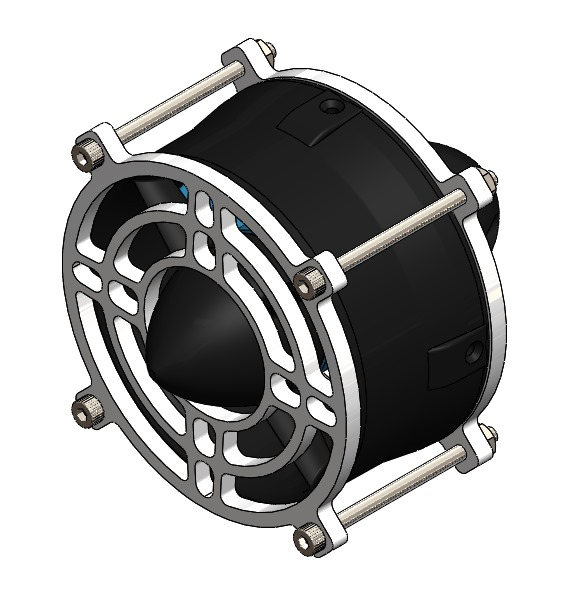
\includegraphics[width=0.6\columnwidth]{Sections/3Safety/images/shrouded_thruster.jpeg}
    \caption{Shrouded Thrusters.}
    \label{fig:shrouds}
\end{figure}

Each thruster operating in the aquatic environment is protected by a fuse to minimize electrical shock risks and prevent damage. For efficient heat dissipation, converters are positioned outside the canister and fully insulated, while heat-conducting components inside the canister are attached to its walls to create a heat sink effect. This design effectively manages temperatures and ensures optimal system performance.
